\documentclass[12pt,a4paper]{article} %Tipo de documento

%Algunos paquetes nesesarios, deben de ir en preambulo las paqueterias.
\usepackage[spanish]{babel} 
\usepackage[utf8]{inputenc}
\usepackage[numbers,sort&compress]{natbib} %Para la bibliografía
\usepackage{graphicx} %Para incluir figuras
\usepackage{amsfonts}
\usepackage[left=2cm,right=2cm,top=2cm,bottom=2cm]{geometry}
\usepackage{listings}
\usepackage[usenames,dvipsnames]{color}

\lstset{ 
  language=R,
  basicstyle=\scriptsize\ttfamily,
  numbers=left,
  numberstyle=\tiny\color{Blue},
  stepnumber=1,
  numbersep=5pt,
  backgroundcolor=\color{white},
  showstringspaces=false,
  showtabs=false,
  frame=single,
  rulecolor=\color{black},
  tabsize=2,
  captionpos=b,
  breaklines=true,
  breakatwhitespace=false,        
  keywordstyle=\color{RoyalBlue},
  commentstyle=\color{YellowGreen},
  stringstyle=\color{ForestGreen}
}


\title{Matemáticas Computacionales \\ Práctica 1: Gráficas de curvas en R} %Título del documento
\author{Profesor: Ángel Isabel Moreno Saucedo \\ Semestre Febrero - Junio 2021} %Autor del documento
\date{}

%Hasta aquí es el preambulo, sigue el documento
\begin{document}

\maketitle %Para crear el título del documento

\section{Introducci\'{o}n}\label{sec:intro} %Sección del documento referenciado con 'intro'

En esta primera práctica se hará una de las cosas básicas al momento de aprende R. Se repasaran las curvas en $\mathbb{R}^2$ vistas en primer semestre en la materia de Geometría Analítica\citep{geometria}. Se graficarán curvas como la recta, parábola, circunferencia, elipse e hipérbola.

\section{Curvas de $\mathbb{R}^2$} \label{sec:curvas}

\subsection{Línea recta} \label{subsec:linearecta}

Partiendo de la ecuación general de la linea recta
\begin{equation}
Ax + By + C = 0, \label{eq:recta}
\end{equation}
se graficará en R. La ecuación (\ref{eq:recta}) se utilizara en su forma pendiente intersección para poder codificar más facil.
\begin{equation}
y = mx + b \label{eq:pendienteinterseccion}
\end{equation}

Hay que pensar en lo datos que ocupamos para gráficar una recta que son la pendiente $m$ y la intersección en el ejes de las ordenadas $b$. Estos dos datos son suficientes para gráficar la recta. Ahora veamos algo de código.

\begin{table}[htpb]
	\begin{lstlisting}
		m <- 3 #pendiente
		b <- 2 #interseccion

		#funcion de la linea recta
		f <- function(m, b, x){
		  return(m * x + b)
		}

		x <- seq(-5, 5, 1)#vector de -5 a 5
		y <- f(m, b, x) #evaluamos

		plot(x, y) #graficamos
	\end{lstlisting}
	\caption{Primer código en R para gráficar una recta.}
	\label{alg:recta0}
\end{table}

\newpage
Si ejecutamos el código anterior en R obtenemos la figura (\ref{fig:recta0}). Observe que solo tenemos graficados puntos, esto es por que la función \texttt{plot()} tiene por default gráficar puntos. Para que nos gráfique líneas tenemos que ponerle la opción ``\texttt{l}" que es de \texttt{line}, ya que andamos ahí vamos a agregar los nombres a los eje y las líneas para generar el plano cartesiano y con más puntos en las x.

\begin{figure}
\centering
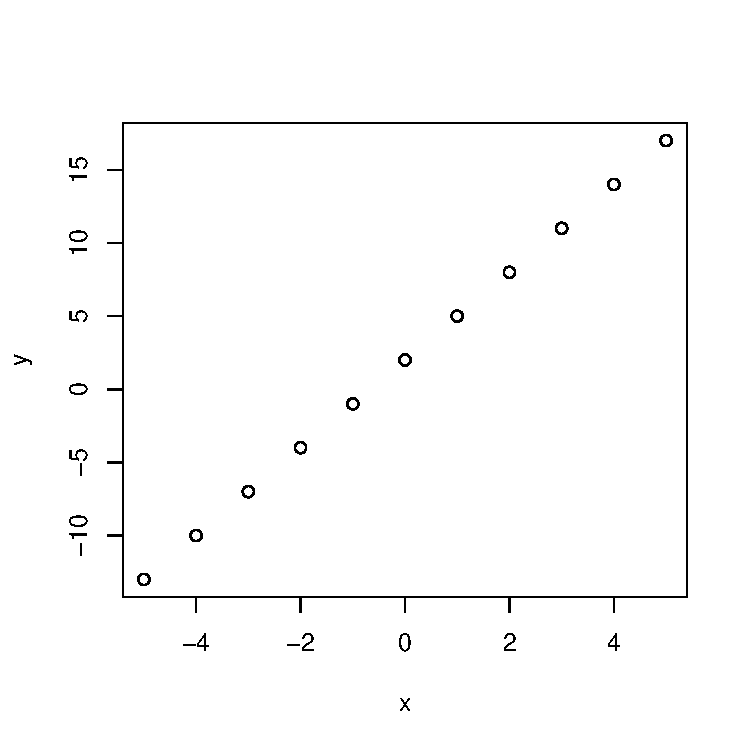
\includegraphics[scale = 0.8]{recta0}
\caption{Gráfico que arroja el primer código ejecutado}
\label{fig:recta0}
\end{figure}

\begin{table}[htpb]
	\lstinputlisting[firstline = 1, lastline = 14]{practica1.R}
	\caption{Código actualizado en R para gráficar una recta.}
	\label{alg:recta1}
\end{table}

\begin{figure}
\centering
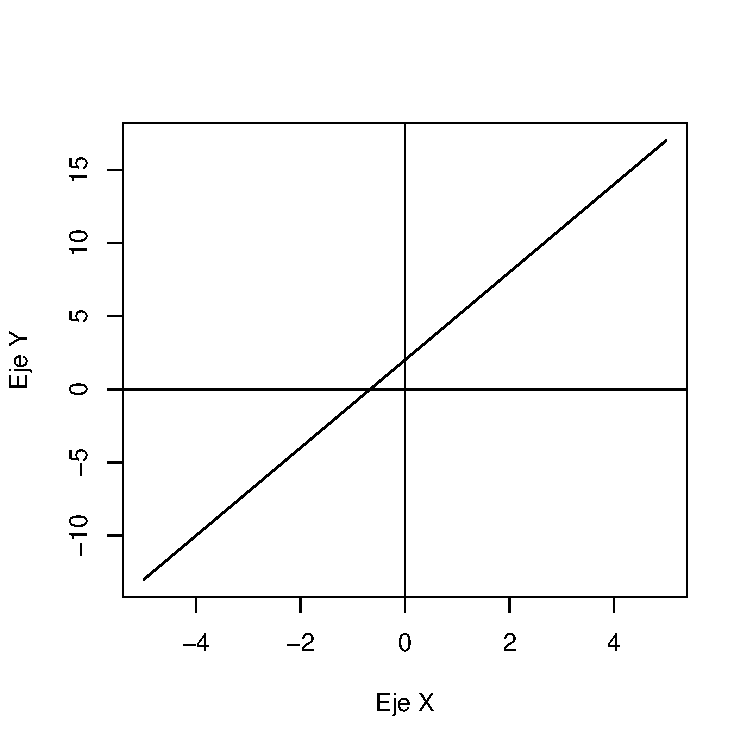
\includegraphics[scale=0.8]{recta1}
\caption{Línea recta con pendiente 3 y pasa por la intersección en 2.}
\label{fig:recta1}
\end{figure}

Agregando como argumento \texttt{type = ``l'', xlab = ``Eje X'', ylab = ``Eje Y''} en la función \texttt{plot()} dibuja la gráfica con lineas en lugar de puntos, Eje X como nombre en el eje de las x y Eje Y como nombre del eje Y. Esto se muestra en la figura (\ref{fig:recta1})

\subsection{Parábola} \label{subsec:parabola}

Para gráficar la parábola lo haremos de otra forma distinta que sera utilizando la ecuación (\ref{eq:parabola}), si forma general. Veamos como lo codificaremos.
\begin{equation}
y = Ax^2 + Bc + C \label{eq:parabola}
\end{equation}

\begin{table}[htpb]
	\lstinputlisting[firstline = 16, lastline = 25]{practica1.R}
	\caption{Código en R para gráficar una parábola.}
	\label{alg:parabola}
\end{table}

\begin{figure}
\centering
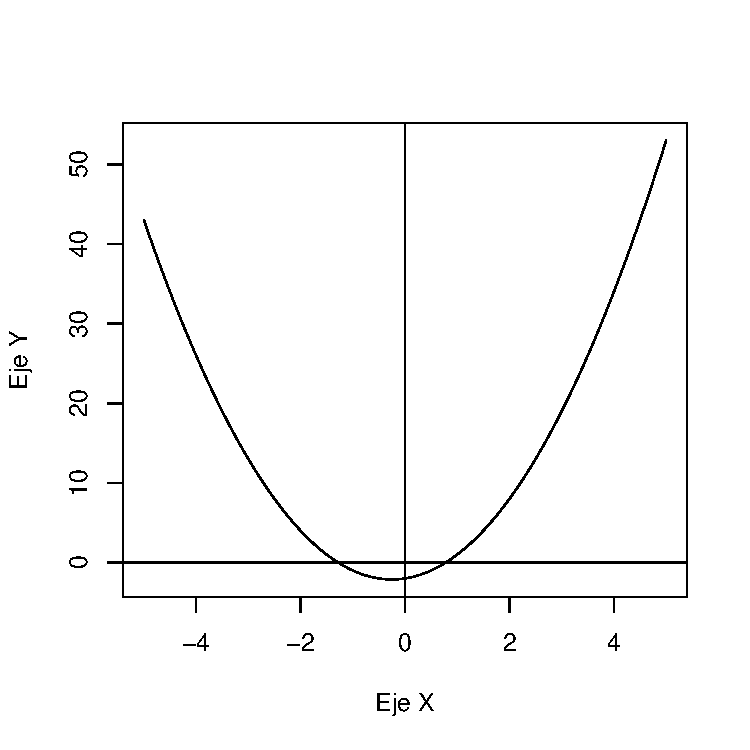
\includegraphics[scale=0.8]{parabola1}
\caption{Grafica de la ecuacion $y = 2x^2 + x - 2$.}
\label{fig:parabola}
\end{figure}

El código no cambia mucho al de la recta, se utiliza las misma funciones. La figura (\ref{eq:parabola}) muestra la gráfica de la ecuación $y = 2x^2 + x - 2$.

\newpage
\subsection{Circunferencia} \label{subsec:circunferencia}

Dada la ecuación ordinaria de circunferencia
\begin{equation}
(x - h)^2 + (y - k)^2 = r^2, \label{eq:circunferencia}
\end{equation}
donde $(h, k)$ es el centro y $r$ es el radio. Utilizando estos datos graficaremos la circunferencia. Primero la ecuación (\ref{eq:circunferencia}) la despejaremos con respecto a $y$ obteniendo las dos ecuaciones:
\begin{equation}
y = k \pm \sqrt{r^2 - (x - h)^2}, \label{eq:circdespejada}
\end{equation}
restringiendo el dominio en $x \in [h - r, h + r]$. Se codifica una función que reciba todos estos datos como entrada y arroje como salida la gráfica de la circunferencia con centro en $(h, k)$ y radio $r$.

El código del cuadro (\ref{alg:circunferencia}) se programa una función llamada \texttt{circunferencia(h, k, r)}. Note que se agrega una validación para $r > 0$ y sí $r = 0$ entonces la gráfica es un punto en $(h, k)$, en otro caso es una circunferencia con el dominio: $x \in [h - r, h + r]$. Se evalúa en en dominio dado obteniendo \texttt{ypositiva} y \texttt{ynegativa} con las ecuaciones en (\ref{eq:circdespejada}). Se agrega adicionalmente dos argumentos mas \texttt{xlim = c(h - (r + 1), h + (r + 1))} y \texttt{ylim = c(k - (r + 1), k + (r + 1))} en la función \texttt{plot()} para controlar los limites de los ejes coordenados, la función \texttt{lines(x, ynegativa, type = ``l'')} añade en el gráfico existente la linea generada por los vectores $(x, ynegativa)$ y \texttt{points(x = h, y = k, col = ``red'')} agrega el centro de la circunferencia con color rojo. La figura (\ref{fig:circunferencia}) muestra la salida del código.

\begin{table}[htpb]
	\lstinputlisting[firstline = 28, lastline = 50]{practica1.R}
	\caption{Código actualizado en R para gráficar una circunferencia.}
	\label{alg:circunferencia}
\end{table}

\begin{figure}
\centering
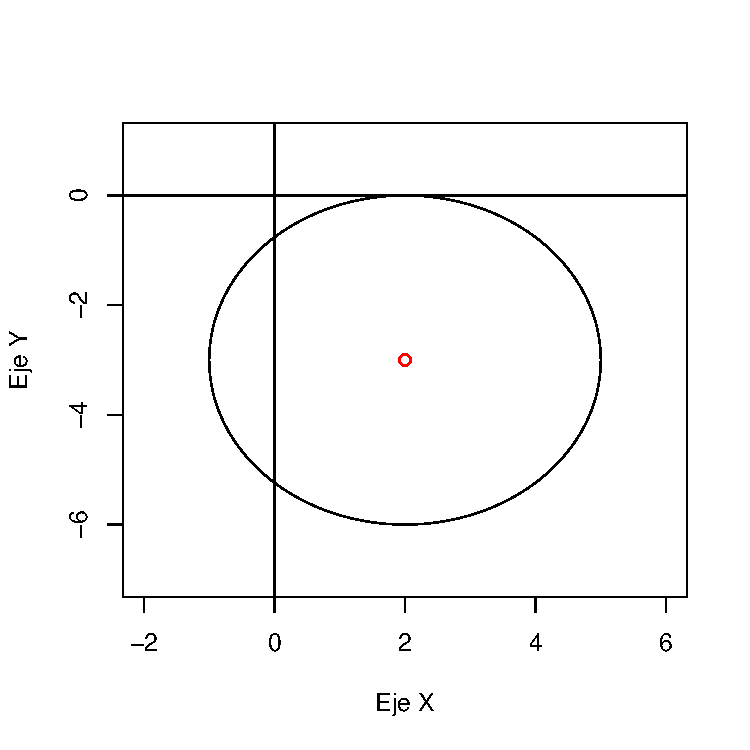
\includegraphics[scale=0.8]{circunferencia}
\caption{Grafica de una circunferencia con centro en (2, -3) y radio 3.}
\label{fig:circunferencia}
\end{figure}

\newpage
\subsection{Elipse}

Partiendo de la ecuación ordinario de la elipse se obtiene despejando con respecto a $y$:
\begin{equation}
y = k \pm \sqrt{b^2 - \frac{b^2}{a^2}(x - h)^2} \label{eq:elipse}
\end{equation}
con dominio $x \in [h - a, h + a]$ ó $x \in [h - b, h + b]$ según el caso. El código es el siguiente:

\begin{table}[htpb]
	\lstinputlisting[firstline = 53, lastline = 82]{practica1.R}
	\caption{Código actualizado en R para gráficar una elipse.}
	\label{alg:elipse}
\end{table}

\begin{figure}
\centering
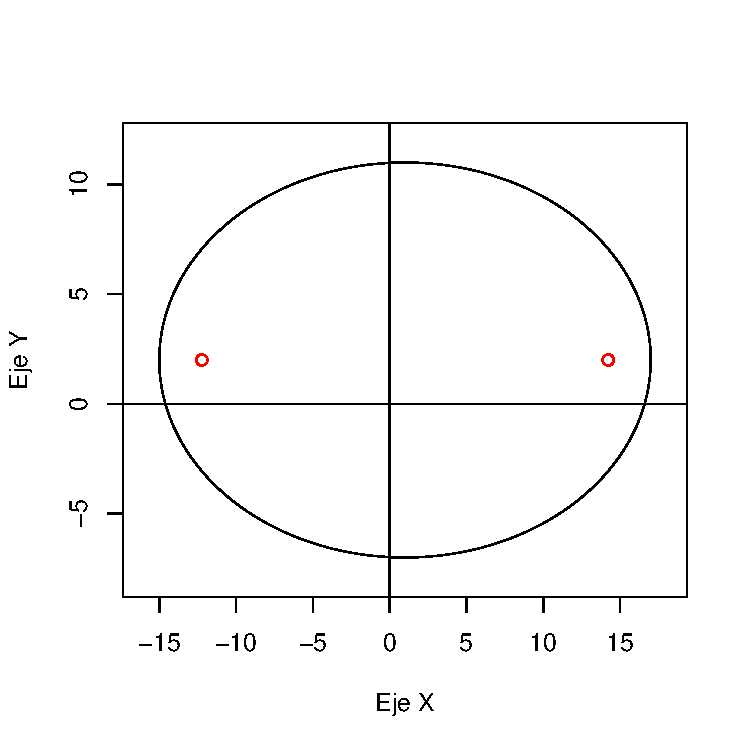
\includegraphics[scale=0.8]{elipse}
\caption{Grafica de una elipse horizontal con centro en (1, 2), $a = 16$ y $b = 9$.}
\label{fig:elipse}
\end{figure}

La función \texttt{elipse(h, k, a, b, horizontal)} recibe en entrada el centro de una elipse $(h, k)$, los valores de las constantes $a$ y $b$, y una variable booleana "\texttt{horizontal}" donde si es una elipse horizontal entonces \texttt{horizontal = TRUE}. Se valida si $a > b$ y si es horizontal (lineas 2 y 4), dependiendo si es horizontal o no el dominio cambia y en los calculos de los vectores \texttt{ypositiva} y \texttt{ynegativa}, se intercambian $a$ y $b$. Las lineas para gráficar son similares que en la circunferencia solo que en esta gráfica agregamos los focos con la línea \texttt{points(x = c(h - c, h + c), y = c(k, k), col = ``red'')} o \texttt{points(x = c(h, h), y = c(k - c, k + c), col = ``red'')} según el caso si es horizontal o no.

\newpage
\subsection{Hipérbola}

Para la hipérbola utilizaremos dos formas para graficarla. Si la hipérbola es horizontal, se utilizara la ecuación:
\begin{equation}
y = k \pm \sqrt{\frac{b^2}{a^2}(x - h)^2 - b^2}, \label{eq:hiperbolah}
\end{equation}
el dominio para gráficar considerado es $x \in [h - (a + 3), h - a] \cup [h + a, h + (a + 3)]$ y para una hipérbola vertical evaluaremos con el rango y utilizando la ecuación:
\begin{equation}
x = h \pm \sqrt{\frac{b^2}{a^2}(y - k)^2 - b^2}, \label{eq:hiperobolav}
\end{equation}
con rango de evaluación $y \in [k - (a + 3), k - a] \cup [k + a, k + (a + 3)]$.

El código del cuadro (\ref{alg:hiperbola}) crea una función \texttt{hiperbola(h, k, a, b, horizontal)} con los parámetros similares a los de la elipse, validación si es una hipérbola horizontal o no, si vamos a evaluar con dominio o rango y las lineas para gráficar idénticas a la de elipse. La figura (\ref{fig:hiperbola}) muestra una parte de la hipérbola, la otra parte de la hipérbola la veremos en la tarea.

\begin{table}[htpb]
	\lstinputlisting[firstline = 84, lastline = 112]{practica1.R}
	\caption{Código actualizado en R para gráficar una hipérbola.}
	\label{alg:hiperbola}
\end{table}

\begin{figure}
\centering
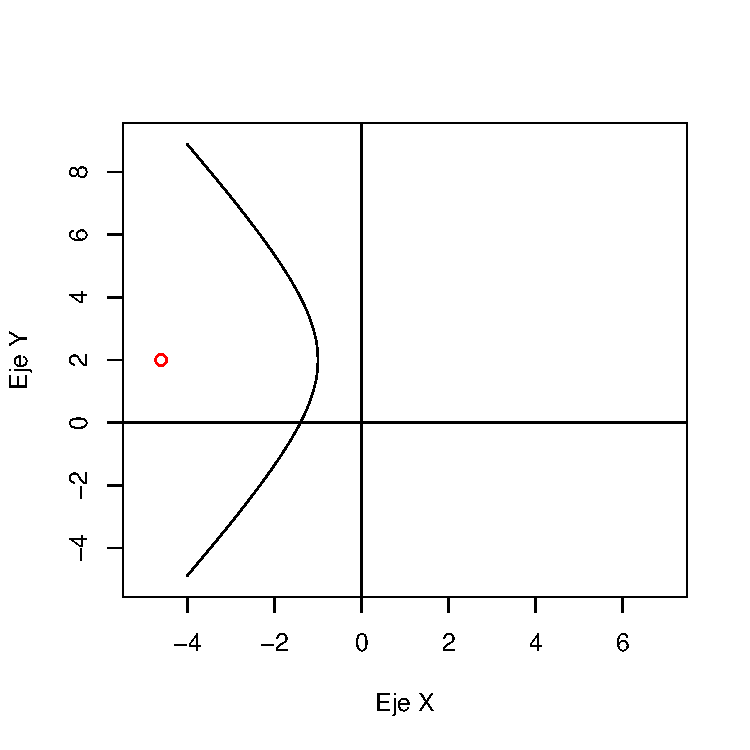
\includegraphics[scale=0.75]{hiperbola}
\caption{Grafica de una hipérbola sobre el eje X con centro en (1, 2), $a = 2$ y $b = 3$.}
\label{fig:hiperbola}
\end{figure}

\section{Tarea}

Termine de dibujar la otra parte de la hipérbola, haga dos gráficas de cada curva agregue en el código lo que ocupe para que al ejecutarse se creen todas la gráficas. Diseñe un reporte de la practica añadiendo estos dibujos con su correspondiente caption junto con la definición de cada curva, puede utilizar el libro de geometria analitica\citep{geometria} para estas definiciones. El codigo guardelo en su repositorio de github. Agregue en la referencias la liga de su repositorio.\citep{repositorio}


%Bibliografia, recuerda siempre que agregues un referencia nueva compilar el archivo BibTex (con F11 en Texmaker), luego el compilar el .tex
\bibliography{biblio}
\bibliographystyle{plainnat}

\end{document}